%%%%%%%%%%%%%%%%%%%%%%%%%%%%%%%%%%%%%%%%%
% University/School Laboratory Report
% LaTeX Template
% Version 4.0 (March 21, 2022)
%
% This template originates from:
% https://www.LaTeXTemplates.com
%
% Authors:
% Vel (vel@latextemplates.com)
% Linux and Unix Users Group at Virginia Tech Wiki
%
% License:
% CC BY-NC-SA 4.0 (https://creativecommons.org/licenses/by-nc-sa/4.0/)
%
%%%%%%%%%%%%%%%%%%%%%%%%%%%%%%%%%%%%%%%%%

%----------------------------------------------------------------------------------------
%	PACKAGES AND DOCUMENT CONFIGURATIONS
%----------------------------------------------------------------------------------------

\documentclass[
	letterpaper, % Paper size, specify a4paper (A4) or letterpaper (US letter)
	10pt, % Default font size, specify 10pt, 11pt or 12pt
]{CSUniSchoolLabReport}

\addbibresource{sample.bib} % Bibliography file (located in the same folder as the template)

%----------------------------------------------------------------------------------------
%	REPORT INFORMATION
%----------------------------------------------------------------------------------------
\usepackage{array}
\title{Experiment Number 5\\The laser beam parameters\\ EP3290} % Report title

\author{Chaganti Kamaraja Siddhartha\\EP20B012} % Author name(s), add additional authors like: '\& James \textsc{Smith}'

\date{\today} % Date of the report

%----------------------------------------------------------------------------------------

\begin{document}

\maketitle % Insert the title, author and date using the information specified above

\begin{center}
	\begin{tabular}{l r}
		Date Performed: & August 16, 2022 \\ % Date the experiment was performed
	\end{tabular}
\end{center}

% If you need to include an abstract, uncomment the lines below
%\begin{abstract}
%	Abstract text
%\end{abstract}

%----------------------------------------------------------------------------------------
%	OBJECTIVE
%----------------------------------------------------------------------------------------
\section{Aim}
To determine the various parameters of a laser beam. Beam Divergence \((\theta_o)\), and Beam spot size.
\section{Objectives}
\begin{enumerate}
	\item To understand the concept of laser. 
	\item To explore application areas of laser. 
	\item To calculate the divergence and spot size of the given laser beam. 
\end{enumerate}
% If you have more than one objective, uncomment the below:
%\begin{description}
%	\item[First Objective] \hfill \\
%	Objective 1 text
%	\item[Second Objective] \hfill \\
%	Objective 2 text
%\end{description}
\section{Apparatus}
\begin{enumerate}
	\item He-Ne gas laser
	\item Light detector with power output
	\item Constant Power supply
	\item Meter scale
\end{enumerate}
\section{Theory}
\subsection{Laser}
The term LASER is the acronym for Light Amplification by Stimulated Emission of
Radiation. It is a mechanism for emitting electromagnetic radiation via the process of stimulated
emission. The laser was the first device capable of amplifying light waves themselves. The emitted
laser light is a spatially coherent, narrow low-divergence beam. When the waves(or photons) of a
beam of light have the same frequency, phase and direction, it is said to be coherent . There are
lasers that emit a broad spectrum of light, or emit different wavelengths of light
simultaneously. According to the encyclopedia  of laser physics and technology, beam divergence
of a laser beam is a measure for how fast the beam expands far from the beam waist. A laser beam
with a narrow beam divergence is greatly used to make laser pointer devices. Generally, the beam
divergence of laser beam is measured using beam profiler.
Divergence means “Departure from norm or Deviation”. The beam divergence of laser
beam is the measure of increase of diameter or radius. A laser beam consists of very nearly
parallel light rays, the beam diameter increases far more slowly with distance from the light
source as compare to the light beam from a other light sources.
\subsection{Beam Spot Size}
Beam Diameter is defined as the distance across the center of the beam for which
the irradiance (I) equals \(\frac{1}{e^2}\) of the maximum irradiance. The spot size of the beam if the radial
distance from the center of maximum irradiance to the \(\frac{1}{e^2}\)  points.
\subsection{Beam Divergence} 
The beam divergence of an electromagnetic beam is an angular mea- sure of the
increase in beam diameter with distance from the optical aperture from which the electromagnetic
beam emerges. 
\subsection{Irradiance distribution I(x,y) and Power transmitted}
The irradiance distribution I(x,y) as a function of the Cartesian coordinates (x,y)
measured from the beam center perpendicular to the direction of propagation is given by
\begin{gather}
	I(x,y) = \frac{2P_{o}}{\pi \omega_{o} ^{2}}\exp [{-2\frac{x^{2}+y^2 }{\omega_o ^2}}]
\end{gather}
Power transmitted past a knife-edge blocking off all points for which x \(\leq\)a is, therefore, given by,
\begin{gather}
	P = \int_{-\infty }^{\infty } \int_{-\infty }^{\infty }  I(x,y) dx dy = \frac{P_{o} }{2} erfc(\frac{a \sqrt{2} }{\omega_{o} })
\end{gather}
It is easy to show that the points with 25 \% and 75 \% of relative powers are located at distances equal to the probable error \(e_p\) \((e_p \approx 0.6745 \omega^\prime )\) on either side of the gaussian distribution, maximum Hence, \(\omega^\prime \)  can be obtained from the relative  power of knife-edge position curve and beam spot size \((2 \omega_{o} = 4 \omega^\prime )\)  can be calculated. \\
\textbf{Divergence}: \(\theta_o  = \frac{1}{\sqrt{2D} }(\omega_3 ^2 - 2 \omega_2 ^2 + \omega_1 ^2 )^\frac{1}{2}\) \\
\textbf{Spot Size} = \(\frac{\lambda}{\pi \theta_o}\) \\
\textbf{Location of Beam Radius}: z = \(\frac{\omega_1 ^2 - \omega_0 ^2 }{\theta_o}\) 
\section{Observations}
\subsection{Measurements with z = 150 mm}
(To determine \(\omega_1\) ):
\begin{figure}[H] % [H] forces the figure to be placed exactly where it appears in the text
	\centering % Horizontally center the figure
	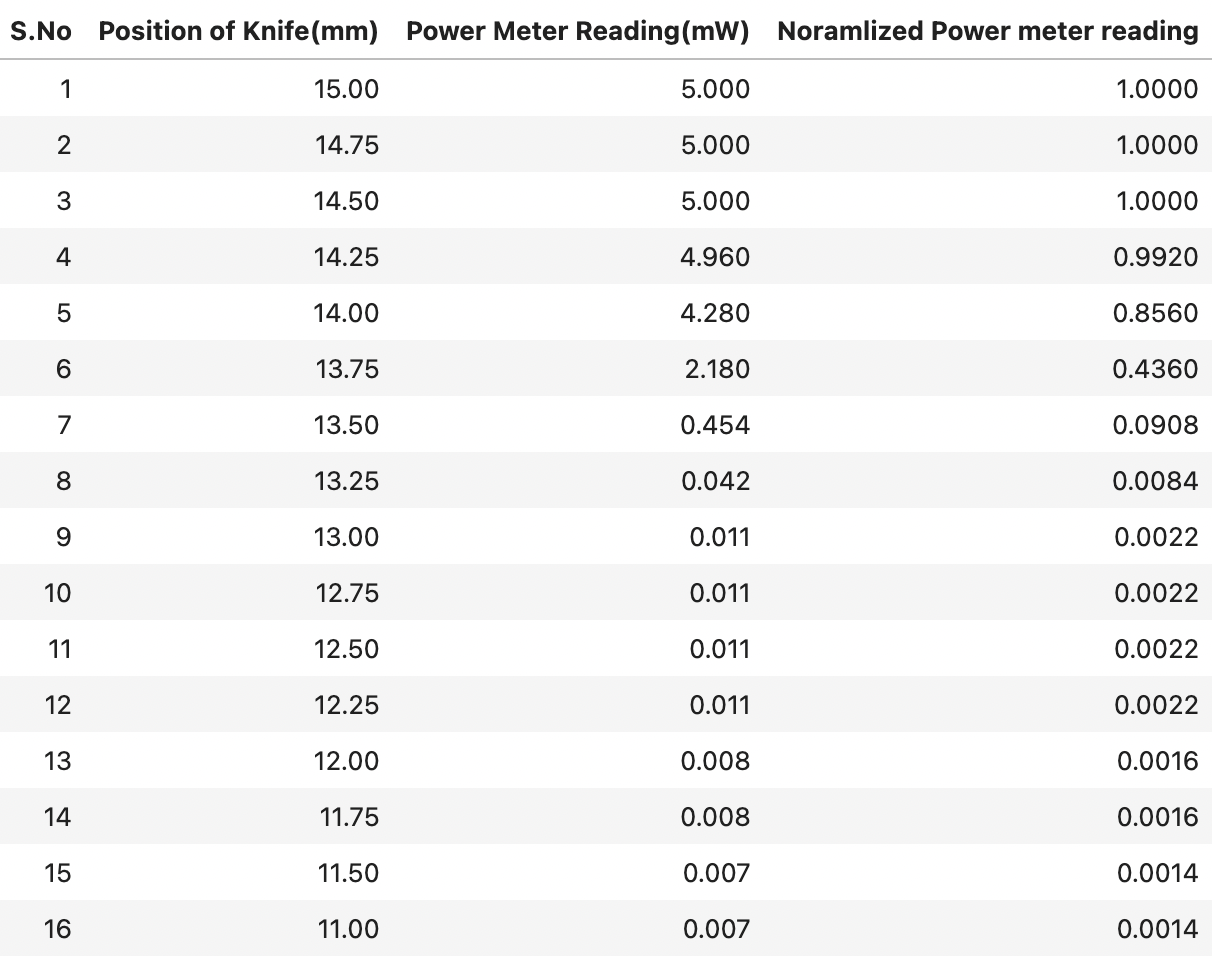
\includegraphics[width=1.1\textwidth]{data1} % Include the figure
	\caption{Experimental Data 1}
\end{figure}
\begin{figure}[H] % [H] forces the figure to be placed exactly where it appears in the text
	\centering % Horizontally center the figure
	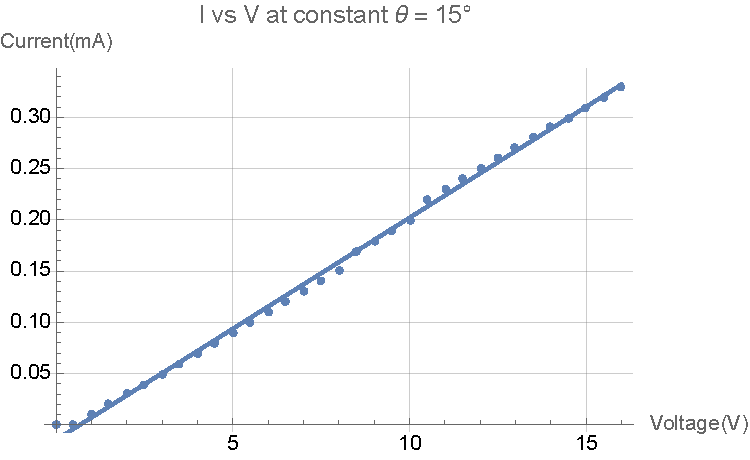
\includegraphics[width=1\textwidth]{graph1} % Include the figure
	\caption{Graph 1}
\end{figure}
\newpage
\subsection{Measurements with z = 300 mm}
To determine \(\omega_2\) :
\begin{figure}[H] % [H] forces the figure to be placed exactly where it appears in the text
	\centering % Horizontally center the figure
	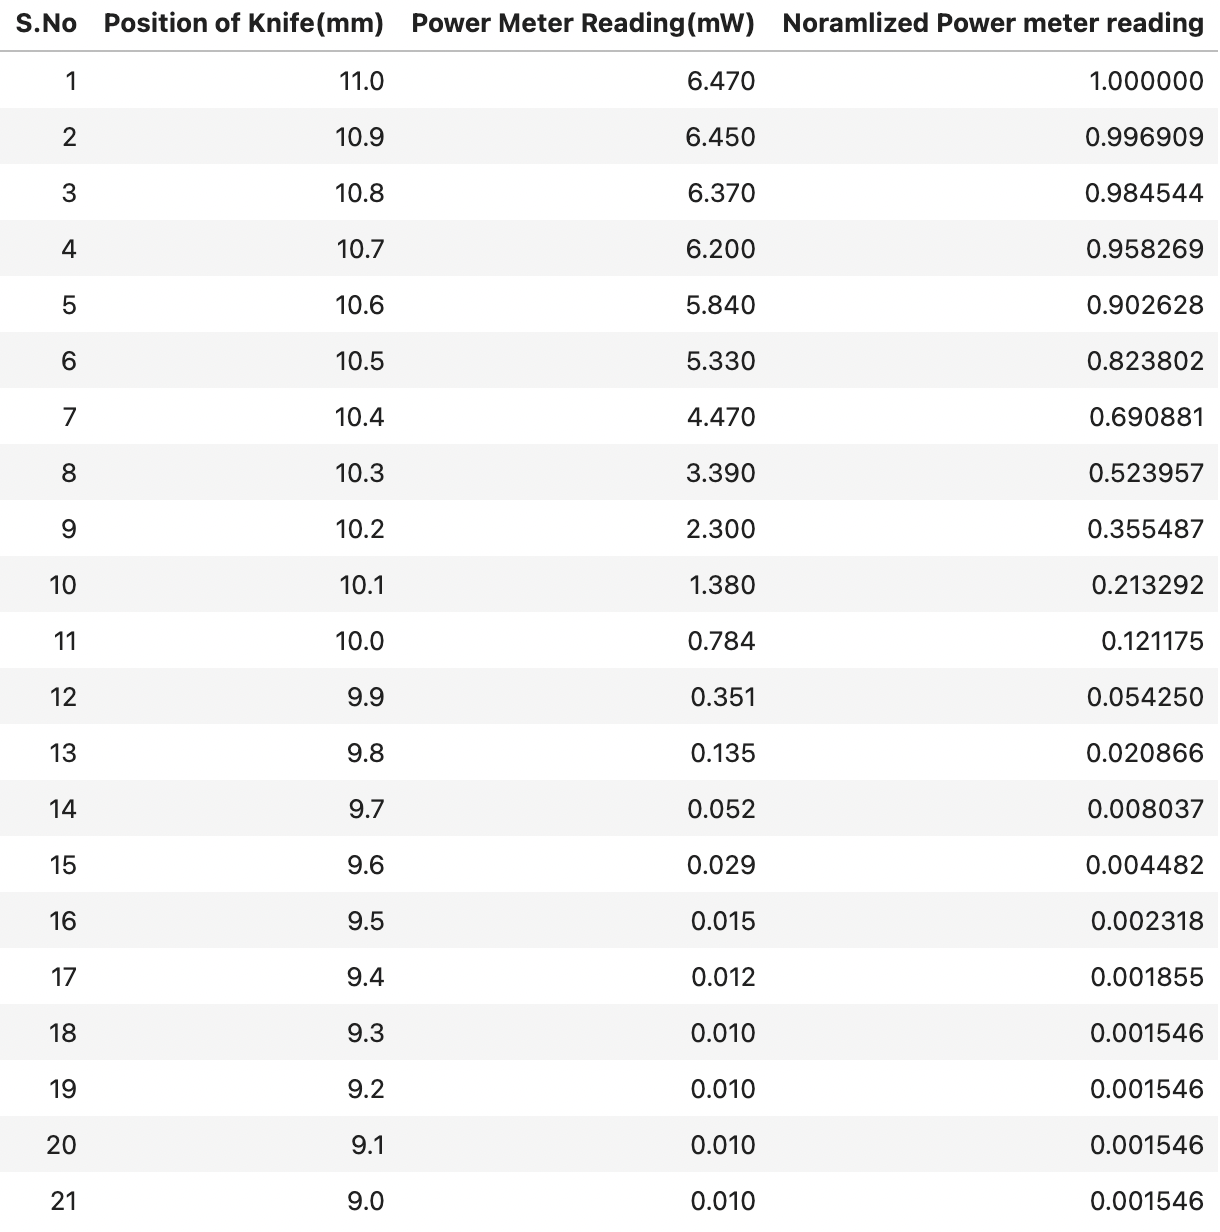
\includegraphics[width=1.1\textwidth]{data2} % Include the figure
	\caption{Experimental Data 2}
\end{figure}
\begin{figure}[H] % [H] forces the figure to be placed exactly where it appears in the text
	\centering % Horizontally center the figure
	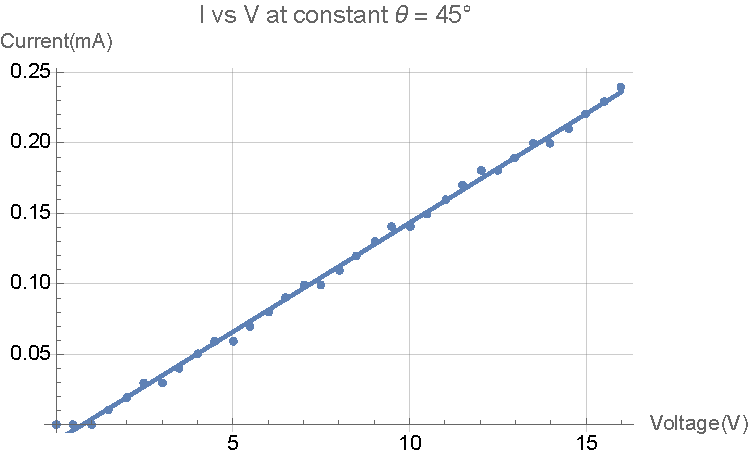
\includegraphics[width=1\textwidth]{graph2} % Include the figure
	\caption{Graph 2}
\end{figure}
\newpage
\subsection{Measurements with z = 450 mm}
To determine \(\omega_3\) 
\begin{figure}[H] % [H] forces the figure to be placed exactly where it appears in the text
	\centering % Horizontally center the figure
	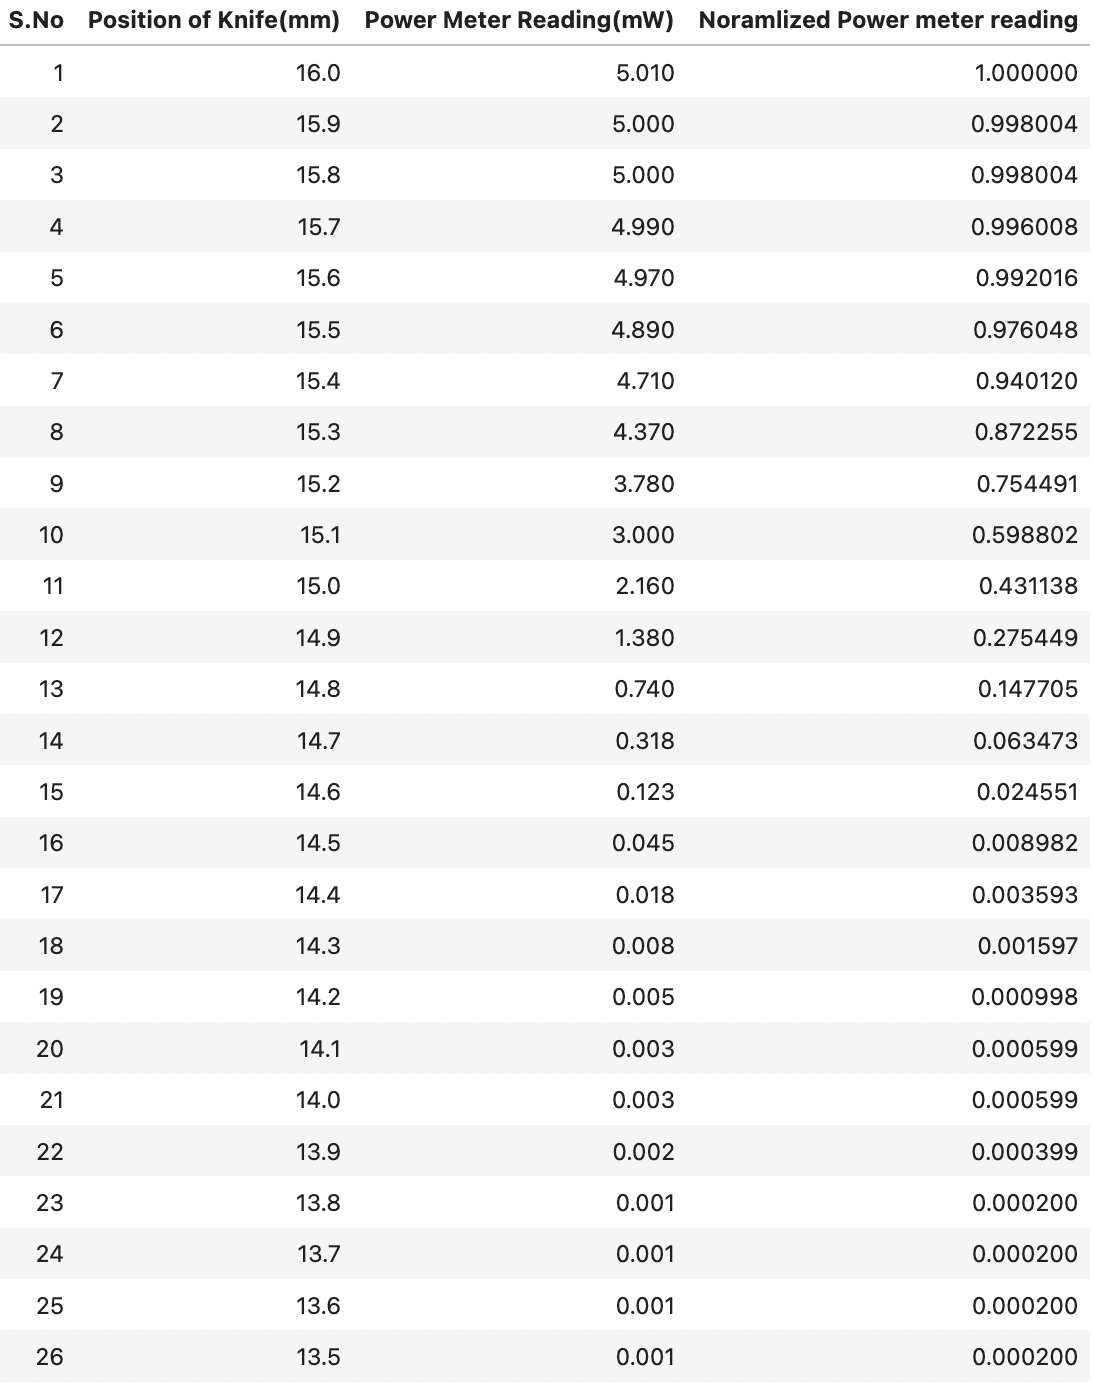
\includegraphics[width=1\textwidth]{data3} % Include the figure
	\caption{Experimental Data 3}
\end{figure}
\begin{figure}[H] % [H] forces the figure to be placed exactly where it appears in the text
	\centering % Horizontally center the figure
	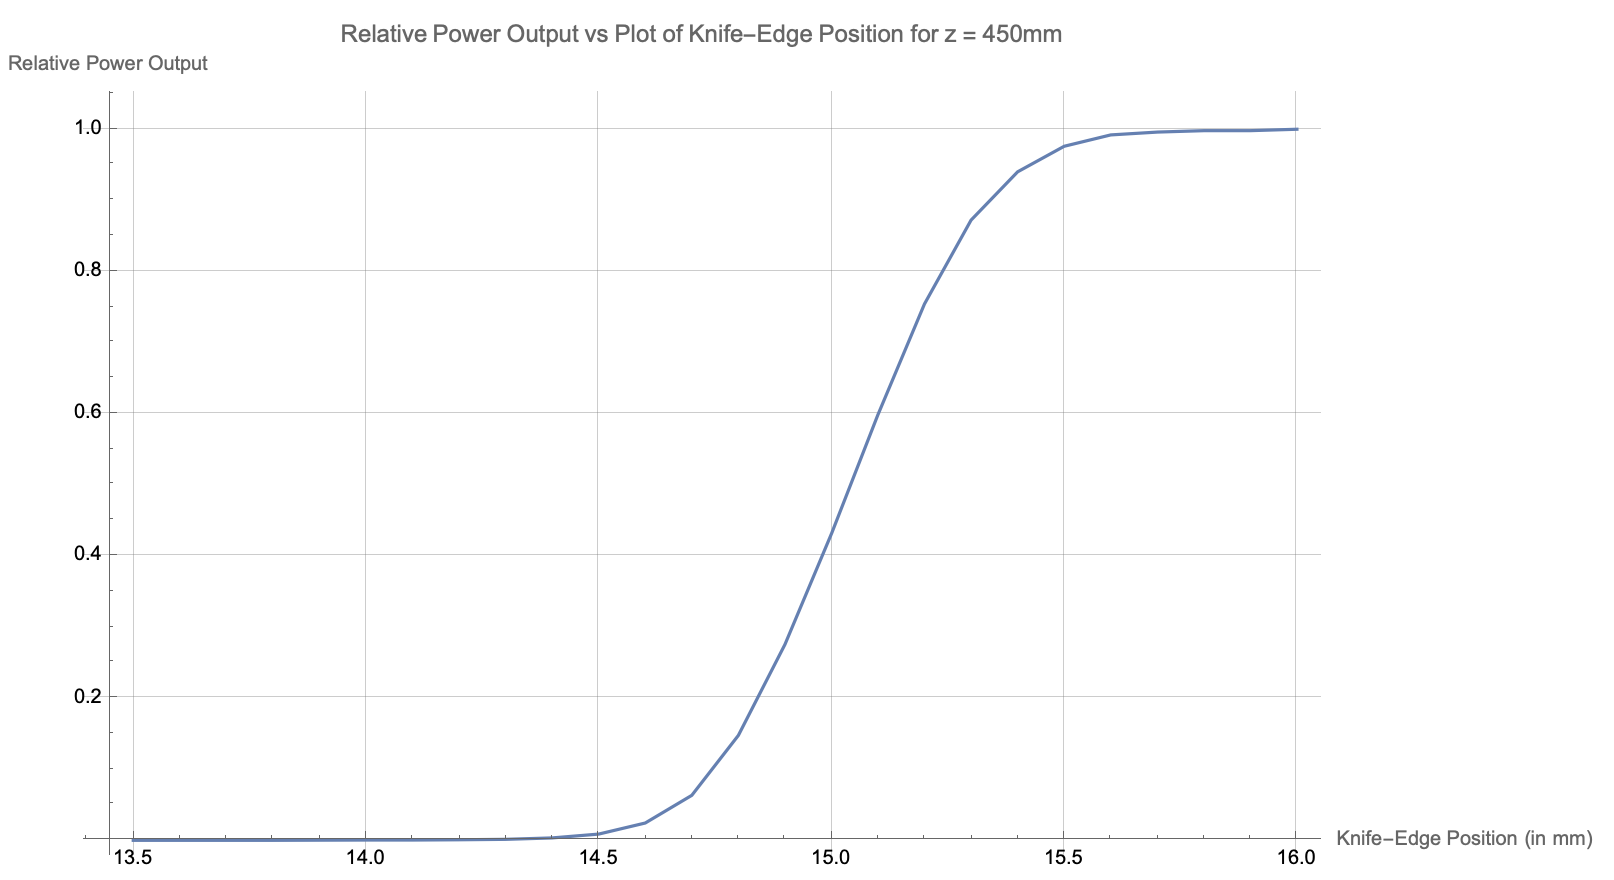
\includegraphics[width=1\textwidth]{graph3} % Include the figure
	\caption{Graph 3}
\end{figure}
\section{Calculations}
\subsection{For z = 150 mm}
75\% power at $x_{75} $ = 14.1mm
25\% power at $x_{25} $= 13.65mm
\[
	2 \times error = \left\vert x_{75} - x_{25}\right\vert \implies error  \frac{0.45}{2}  \approx 0.225 mm
\]
\[
	\omega_1 = \frac{0.225}{0.6745} /approx 0.333 mm
\]
\subsection{For z = 300 mm}
75\% power at $x_{75} $ = 10.45mm
25\% power at $x_{25} $= 10.10mm
\[
	2 \times error = \left\vert x_{75} - x_{25}\right\vert \implies error  \frac{0.35}{2}  \approx 0.175 mm
\]
\[
	\omega_2 = \frac{0.175}{0.6745} /approx 0.259 mm
\]
\subsection{For z = 450 mm}
75\% power at $x_{75} $ = 15.2mm
25\% power at $x_{25} $= 14.9mm
\[
	2 \times error = \left\vert x_{75} - x_{25}\right\vert \implies error  \frac{0.3}{2}  \approx 0.15 mm
\]
\[
	\omega_3 = \frac{0.15}{0.6745} /approx 0.222 mm
\]
\subsection{Divergence}
\[
	\theta_o  = \frac{1}{\sqrt{2 } D}(\omega_3 ^2 - 2 \omega_2 ^2 + \omega_1 ^2 )^\frac{1}{2}
\]
\[
	\theta_o = \frac{1}{\sqrt{2 } 150}(0.222^2 - 2(0.259)^2 +(0.333)^2)^\frac{1}{2} \approx 0.76\times 10^{-3} 
\]
\subsection{Spot size}
\[
	\omega_o = \frac{\lambda}{\pi \theta_o}
\]
\[
	\omega_o = \frac{632.8 nm}{\pi\times  0.76\times 10^{-3} } = 265 \mu m
\]
\subsection{Location of Beam Radius}
\[
	z_o = \frac{(\omega_1^2 - \omega_o^2)^\frac{1}{2}}{\theta_o} = \frac{(0.333^2 - 0.265^2)^\frac{1}{2}}{0.76\times 10^{-3} } = 265.3 mm
\]
\section{Error Analysis}
We measure \(\omega_1\), \(\omega_2\) , \(\omega_3\) with the help of position of knife edge with L.C = 0.02 mm and Power-meter readings with Lc = 0.001mW. 
\subsection{Error in measuring \(\omega_i\) }
\[
	0.6745 \times \omega \times 2 = \left\vert x_{75} - x_{25}   \right\vert 
\]
\[
	2\times 0.6745\times \omega = 2 dx \implies d\omega = \frac{dx}{0.6745}
\]
\[
	\frac{d\omega}{\omega} = \frac{0.02 mm}{0.6745 \times \omega}
\]
\[
	\frac{d\omega_1}{\omega_1} = \frac{0.02}{0.6745 \times 0.333} = 0.089
\]
\[
	\frac{d\omega_2}{\omega_2} = \frac{0.02}{0.6745 \times 0.259} = 0.114
\]
\[
	\frac{d\omega_3}{\omega_3} = \frac{0.02}{0.6745 \times 0.222} = 0.134
\]
\subsection{Error in measuring \(\theta_o\) }
\[
	\frac{d\theta_o}{\theta_o} = \frac{1}{\omega_1^2 -2\omega_2^2 + \omega_3^2}\times \left(\omega_1\times d\omega_1+2\times \omega_2\times d\omega_2+\omega_3\times d\omega_3\right)
\]
\[
	\frac{d\theta_o}{\theta_o} = \frac{1}{0.333^2 - 2\times 0.259^2 + 0.222^2}\times \left(0.333^2\times 0.089+2\times0.259^2\times  0.114+0.222^2\times 0.134\right) 
\]
\[
	\frac{d\theta_o}{\theta_o} = 1.22\%
\]
\subsection{Error in Measurement in Beam Radius \(\omega_o\) }
\[
	\frac{d\omega_o}{\omega_o} = \frac{1}{\pi}\frac{d\theta_o}{\theta_o} = 0.388\%
\]
\subsection{Distance of Beam Radii \(z_o\) }
\[
	\frac{dz_o}{z_o} = \frac{1}{z_o}d(\frac{1}{\theta_o}.\sqrt{\omega_1^2 - \omega_2^2} )
\]
\[
	\frac{dz_o}{z_o} = \frac{1}{z_o}\times \left(\frac{1}{\theta_o^2}d\theta_o \sqrt{\omega_1^2 - \omega_0 ^2} + \frac{1}{\theta_o}\frac{1}{2\sqrt{\omega_1^2 - \omega_o^2} }2(\omega_1d\omega_1 + \omega_{o}d\omega_o )\right)
\]
\[
	\frac{dz_o}{z_o} = \frac{1}{265.3} \times \left(\frac{1}{0.76\times 10^{-3}}\times 1.22\sqrt{0.333^{2}-0.265^2 } +\frac{1}{0.76\times 10^{-3}}\times \frac{1}{2\sqrt{0.333^{2}-0.265^2} }\times 2(0.333^{2}\times 0.089 + 0.265^2\times 0.388)\right)
\]
\[
	\frac{dz_o}{z_o} = 2.12 \%
\]
\section{Conclusion}
\begin{enumerate}
	\item Divergence, \(\theta_o = 0.76\times 10^{-3} \pm 1.22\% \)  
	\item Spot size, \(\omega_o = 265 \mu m \pm 0.38\%\) 
	\item Location of Beam Radius, \(z_o = 265.3 mm \pm 2.12\%\) 
\end{enumerate}
\section{Sources of Error and Precautions}
\begin{enumerate}
\item Massive error is propagated due fo \(\omega_1\),\(\omega_2\) and \(\omega_3\)   . Ensure that the Power vs knife-edge distance graphs qre sufficiently  accurate.
\item Ensure that the laser, knife-edge, and detecter are perfectly with respect to one another so that they form a straight line. 
\item Care should be taken to ensure that the laser beam, after reflection off of the detector does not enter into the laser apparatus or human eyes. 
\end{enumerate}
\end{document}